\documentclass[11pt]{article}

\usepackage[a4paper, margin=1in]{geometry}
\usepackage{graphicx}
\usepackage{listings}
\usepackage{xcolor}
\usepackage{hyperref}

\lstset{
    basicstyle=\ttfamily\small,
    breaklines=true,
    frame=single
}

\title{\textbf{Mr Robot CTF – Penetration Testing Report}}
\author{Joshua Sanctus}
\date{}

\begin{document}

\maketitle
\tableofcontents
\newpage

\section{Overview}

This report documents the exploitation of the Mr Robot CTF machine.  
The objective was to identify vulnerabilities and obtain all three keys.  
The system was successfully compromised through web exploitation, credential discovery, and privilege escalation.

% -------------------------
\section{Methodology}

The following steps were followed:

\begin{itemize}
\item Reconnaissance
\item Enumeration
\item Exploitation
\item Privilege Escalation
\item Post-Exploitation
\end{itemize}

% -------------------------
\section{Reconnaissance}

An Nmap scan was performed to identify open ports and services on the target system.

\begin{lstlisting}
nmap -sC -sV 192.168.109.133
\end{lstlisting}

The scan revealed that HTTP (port 80) and HTTPS (port 443) services were exposed, indicating a web-based attack surface.

As shown in Figure~\ref{fig:nmap}, these services were accessible and provided a starting point for further enumeration.

\begin{figure}[h]
\centering
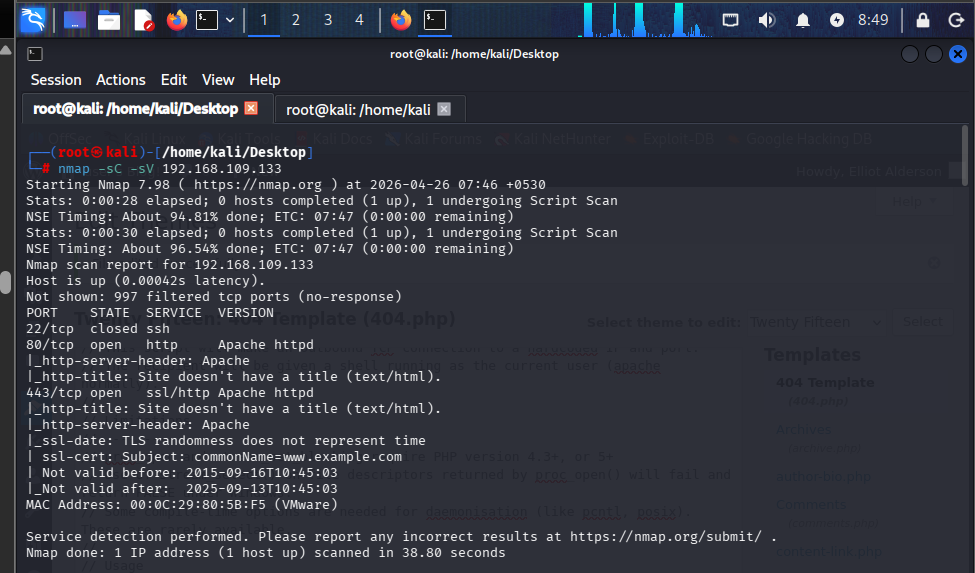
\includegraphics[width=0.6\textwidth]{nmap.png}
\caption{Nmap scan results showing open ports and services}
\label{fig:nmap}
\end{figure}

% -------------------------
\section{Enumeration}

\subsection{Web Enumeration}

The web server was identified as hosting a WordPress application. 
Exploration of the site revealed multiple pages along with a login panel, indicating a potential authentication entry point for further testing.

\subsection{Robots File}

The \texttt{robots.txt} file was examined and revealed sensitive information, including a wordlist and a key file:

\begin{itemize}
\item fsocity.dic
\item key-1-of-3.txt
\end{itemize}

Accessing the key directly:

\begin{lstlisting}
http://192.168.109.133/key-1-of-3.txt
\end{lstlisting}

As shown in Figure~\ref{fig:key1}, the first key was successfully retrieved.

\begin{figure}[h]
\centering
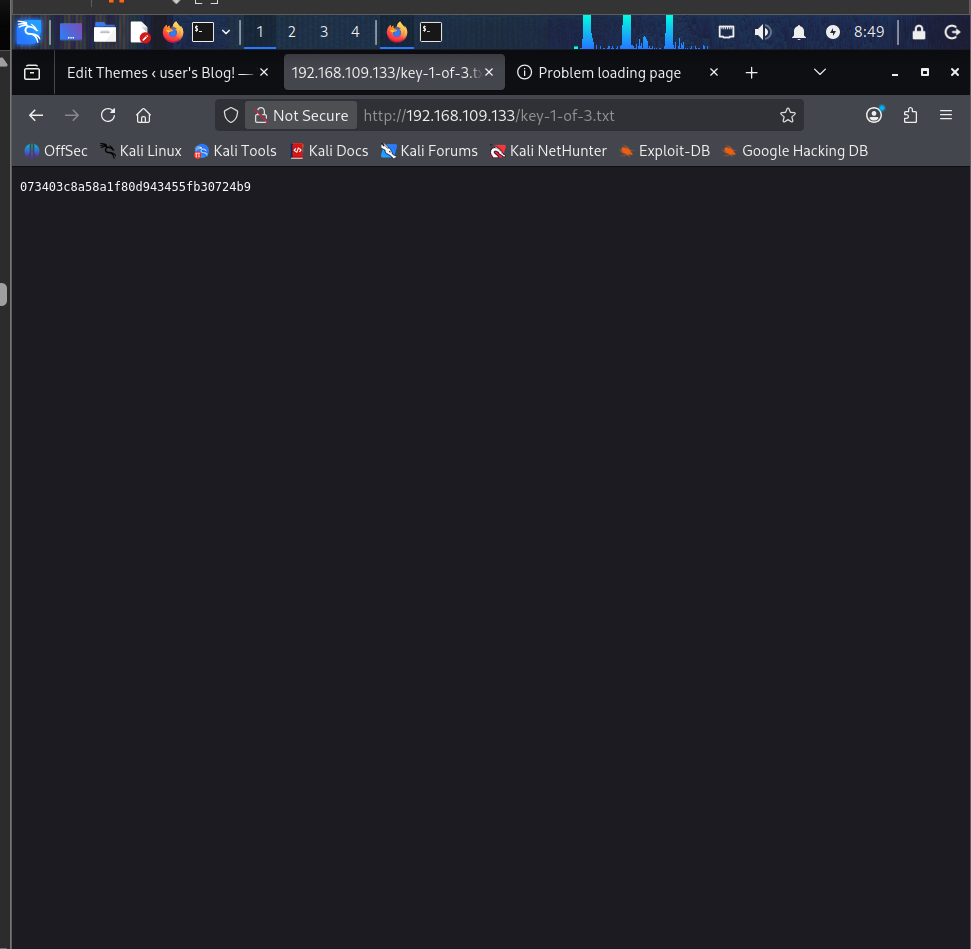
\includegraphics[width=0.6\textwidth]{firstkey.png}
\caption{First key obtained from robots.txt}
\label{fig:key1}
\end{figure}

% -------------------------
\section{Exploitation}

Initial access was obtained by injecting a reverse shell into the WordPress theme editor. Here we are using the 404.php, we replace the contents of the PHP code with the reverse shell code, which can be used to gain access/ 

\begin{figure}[h]
\centering
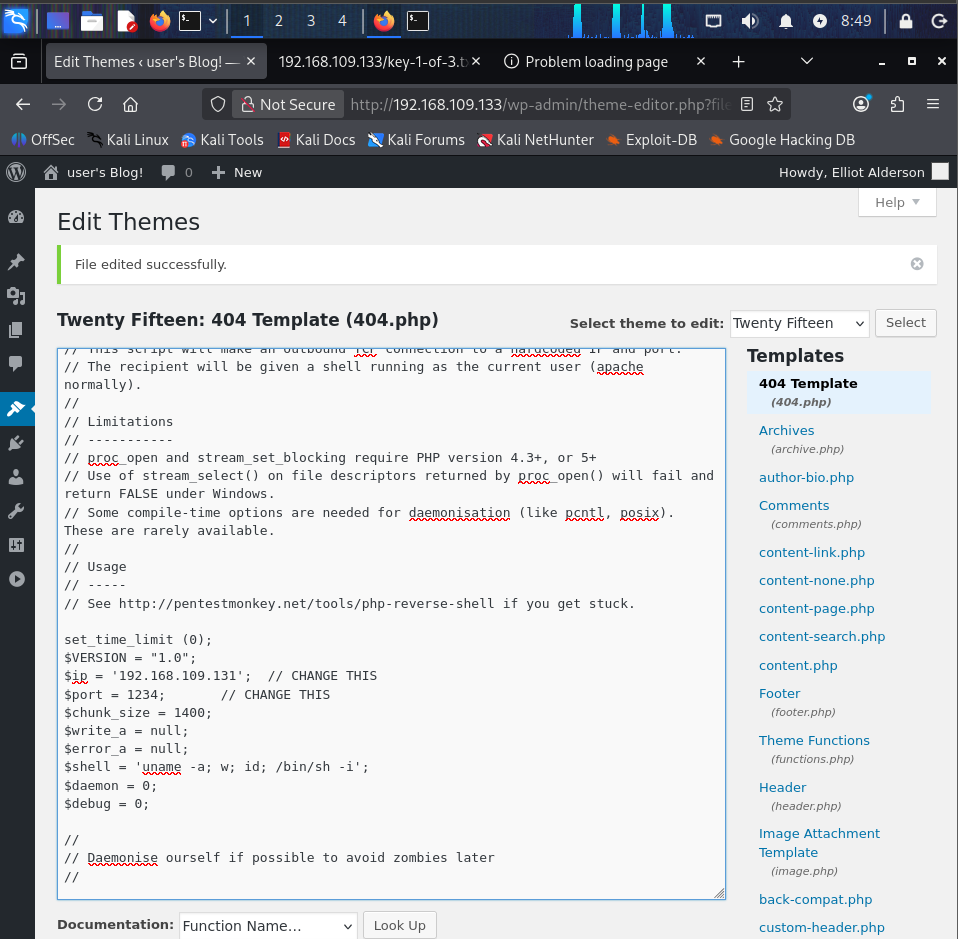
\includegraphics[width=0.7\textwidth]{404.png}
\caption{Editing 404.php's content with the shell code (also in PHP)}
\label{fig:editing}
\end{figure}

A listener was started on the attacker's machine:

\begin{lstlisting}
nc -lvnp 1234
\end{lstlisting}

Once the payload was executed, a connection was received, providing a shell as the \texttt{daemon} user.

As shown in Figure~\ref{fig:exploit}, the reverse shell was successfully established and the second key was retrieved.

\begin{figure}[h]
\centering
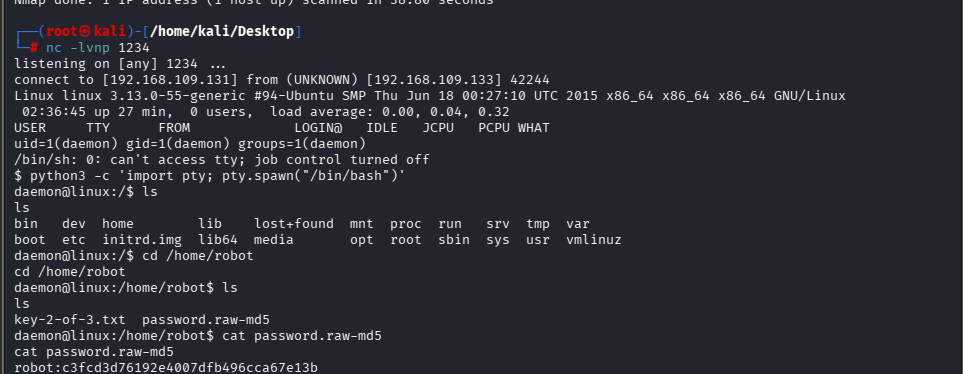
\includegraphics[width=0.9\textwidth]{exploitation_and_2ndkey.png}
\caption{Reverse shell connection and second key retrieval}
\label{fig:exploit}
\end{figure}

% -------------------------
\section{Credential Discovery}

Navigating to the robot user directory revealed a password hash:

\begin{lstlisting}
cat /home/robot/password.raw-md5
\end{lstlisting}

The hash was cracked using Crack Station. Recovered credentials allowed access to the \texttt{robot} user, which can be used to check the privileges the robot user has.

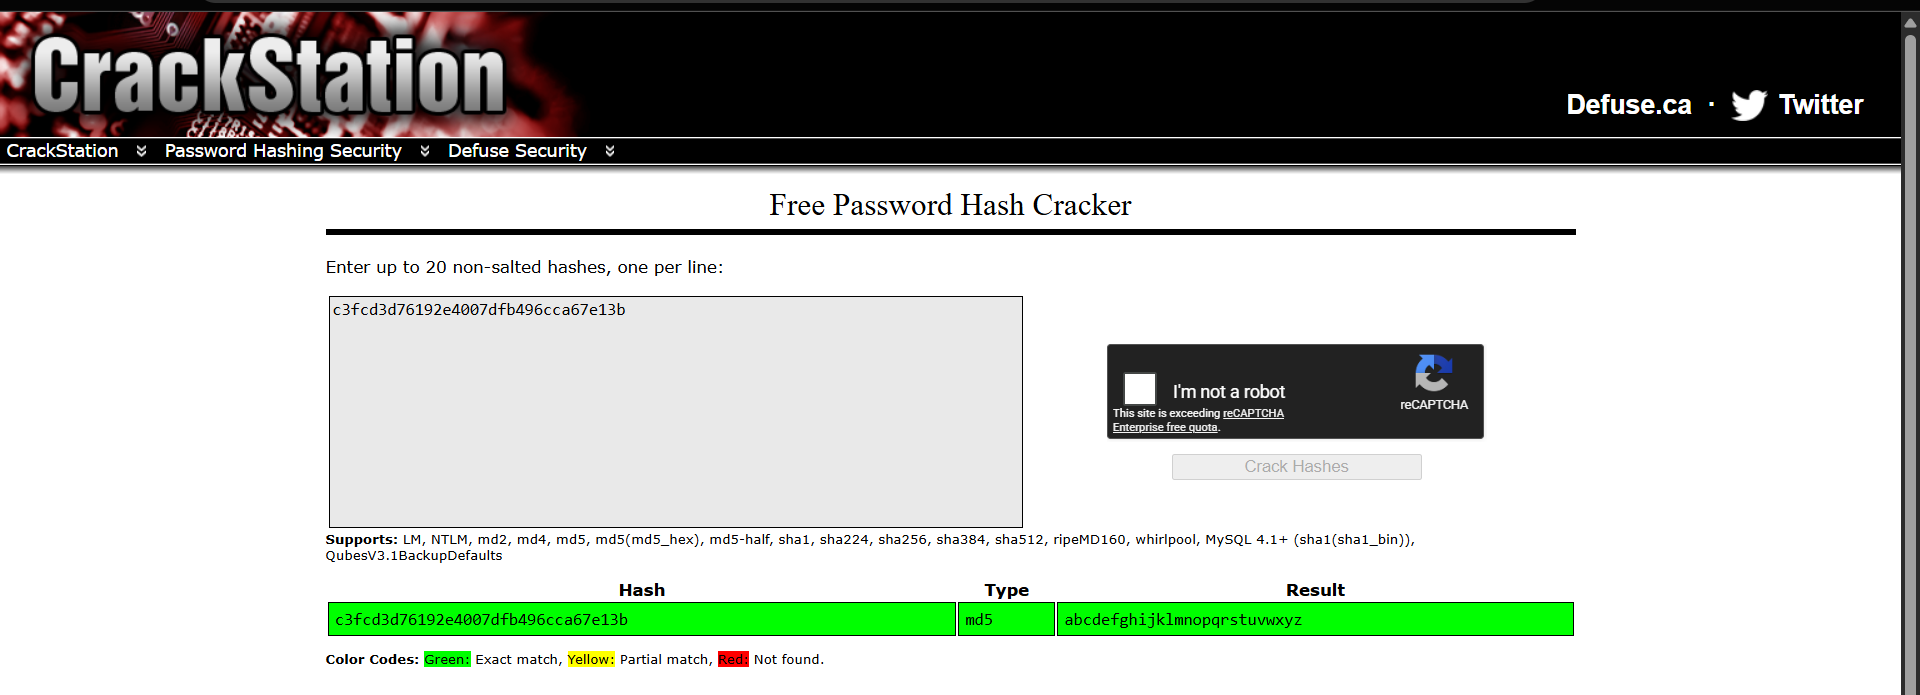
\includegraphics[width=\textwidth]{cracking_hash.png}

% -------------------------
\section{Privilege Escalation}

\subsection{Enumeration}

After obtaining a low-privileged shell, SUID binaries were enumerated to identify potential privilege escalation vectors:

\begin{lstlisting}
find / -perm -4000 -type f 2>/dev/null
\end{lstlisting}

The following binary was identified:

\begin{itemize}
\item /usr/local/bin/nmap
\end{itemize}

As shown in Figure~\ref{fig:suid}, the Nmap binary had the SUID bit set.

\begin{figure}[h]
\centering
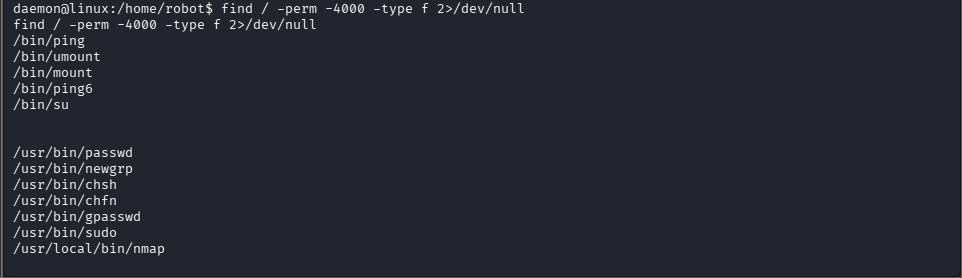
\includegraphics[width=0.9\textwidth]{find_priv_vul.png}
\caption{SUID enumeration showing Nmap binary}
\label{fig:suid}
\end{figure}

Older versions of Nmap support an interactive mode, which can be abused to execute commands with elevated privileges when the binary has SUID permissions.

\subsection{Exploitation}

The identified Nmap binary was executed in interactive mode:

\begin{lstlisting}
nmap --interactive
!sh
\end{lstlisting}

This allowed execution of a shell with root privileges.

As shown in Figure~\ref{fig:root}, root access was successfully obtained, and the final key was retrieved.

\begin{figure}[h]
\centering
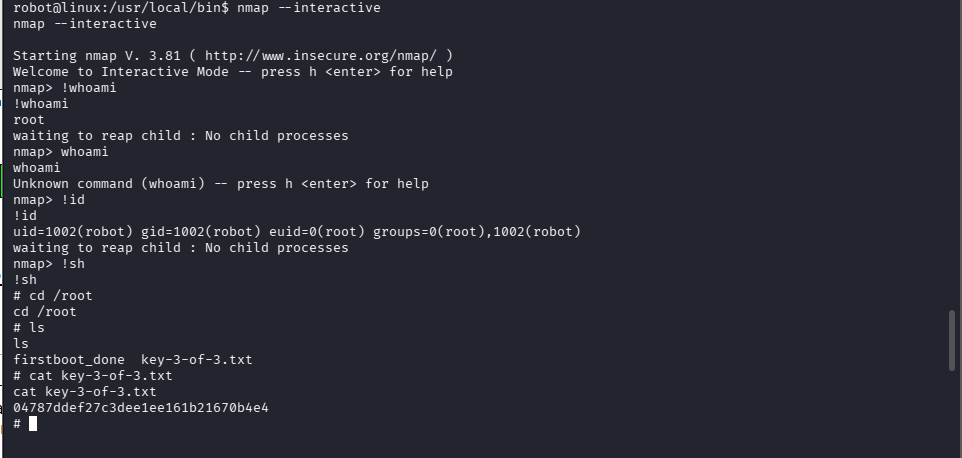
\includegraphics[width=0.9\textwidth]{thirdkey.png}
\caption{Root shell and final key retrieval}
\label{fig:root}
\end{figure}

% -------------------------

\section{Flags Captured}

\begin{itemize}
\item Key 1: 073403c8a58a1f80d943455fb30724b9
\item Key 2: 822c73956184f694993bede3eb39f959
\item Key 3: 04787ddef27c3dee1ee161b21670b4e4
\end{itemize}

% -------------------------
\section{Recommendations}

\begin{itemize}
\item Remove unnecessary SUID permissions from binaries such as Nmap
\item Update outdated software to prevent exploitation
\item Avoid storing passwords using weak hashing algorithms like MD5
\item Restrict access to sensitive WordPress features such as the theme editor
\end{itemize}

% -------------------------
\section{Conclusion}

The system was successfully compromised through multiple vulnerabilities, including insecure configurations and outdated software.  
Proper security practices and system hardening would prevent such attacks.

\end{document}